% Options for packages loaded elsewhere
\PassOptionsToPackage{unicode}{hyperref}
\PassOptionsToPackage{hyphens}{url}
\documentclass[
]{article}
\usepackage{xcolor}
\usepackage{amsmath,amssymb}
\setcounter{secnumdepth}{-\maxdimen} % remove section numbering
\usepackage{iftex}
\ifPDFTeX
  \usepackage[T1]{fontenc}
  \usepackage[utf8]{inputenc}
  \usepackage{textcomp} % provide euro and other symbols
\else % if luatex or xetex
  \usepackage{unicode-math} % this also loads fontspec
  \defaultfontfeatures{Scale=MatchLowercase}
  \defaultfontfeatures[\rmfamily]{Ligatures=TeX,Scale=1}
\fi
\usepackage{lmodern}
\ifPDFTeX\else
  % xetex/luatex font selection
\fi
% Use upquote if available, for straight quotes in verbatim environments
\IfFileExists{upquote.sty}{\usepackage{upquote}}{}
\IfFileExists{microtype.sty}{% use microtype if available
  \usepackage[]{microtype}
  \UseMicrotypeSet[protrusion]{basicmath} % disable protrusion for tt fonts
}{}
\makeatletter
\@ifundefined{KOMAClassName}{% if non-KOMA class
  \IfFileExists{parskip.sty}{%
    \usepackage{parskip}
  }{% else
    \setlength{\parindent}{0pt}
    \setlength{\parskip}{6pt plus 2pt minus 1pt}}
}{% if KOMA class
  \KOMAoptions{parskip=half}}
\makeatother
\usepackage{color}
\usepackage{fancyvrb}
\newcommand{\VerbBar}{|}
\newcommand{\VERB}{\Verb[commandchars=\\\{\}]}
\DefineVerbatimEnvironment{Highlighting}{Verbatim}{commandchars=\\\{\}}
% Add ',fontsize=\small' for more characters per line
\newenvironment{Shaded}{}{}
\newcommand{\AlertTok}[1]{\textcolor[rgb]{1.00,0.00,0.00}{\textbf{#1}}}
\newcommand{\AnnotationTok}[1]{\textcolor[rgb]{0.38,0.63,0.69}{\textbf{\textit{#1}}}}
\newcommand{\AttributeTok}[1]{\textcolor[rgb]{0.49,0.56,0.16}{#1}}
\newcommand{\BaseNTok}[1]{\textcolor[rgb]{0.25,0.63,0.44}{#1}}
\newcommand{\BuiltInTok}[1]{\textcolor[rgb]{0.00,0.50,0.00}{#1}}
\newcommand{\CharTok}[1]{\textcolor[rgb]{0.25,0.44,0.63}{#1}}
\newcommand{\CommentTok}[1]{\textcolor[rgb]{0.38,0.63,0.69}{\textit{#1}}}
\newcommand{\CommentVarTok}[1]{\textcolor[rgb]{0.38,0.63,0.69}{\textbf{\textit{#1}}}}
\newcommand{\ConstantTok}[1]{\textcolor[rgb]{0.53,0.00,0.00}{#1}}
\newcommand{\ControlFlowTok}[1]{\textcolor[rgb]{0.00,0.44,0.13}{\textbf{#1}}}
\newcommand{\DataTypeTok}[1]{\textcolor[rgb]{0.56,0.13,0.00}{#1}}
\newcommand{\DecValTok}[1]{\textcolor[rgb]{0.25,0.63,0.44}{#1}}
\newcommand{\DocumentationTok}[1]{\textcolor[rgb]{0.73,0.13,0.13}{\textit{#1}}}
\newcommand{\ErrorTok}[1]{\textcolor[rgb]{1.00,0.00,0.00}{\textbf{#1}}}
\newcommand{\ExtensionTok}[1]{#1}
\newcommand{\FloatTok}[1]{\textcolor[rgb]{0.25,0.63,0.44}{#1}}
\newcommand{\FunctionTok}[1]{\textcolor[rgb]{0.02,0.16,0.49}{#1}}
\newcommand{\ImportTok}[1]{\textcolor[rgb]{0.00,0.50,0.00}{\textbf{#1}}}
\newcommand{\InformationTok}[1]{\textcolor[rgb]{0.38,0.63,0.69}{\textbf{\textit{#1}}}}
\newcommand{\KeywordTok}[1]{\textcolor[rgb]{0.00,0.44,0.13}{\textbf{#1}}}
\newcommand{\NormalTok}[1]{#1}
\newcommand{\OperatorTok}[1]{\textcolor[rgb]{0.40,0.40,0.40}{#1}}
\newcommand{\OtherTok}[1]{\textcolor[rgb]{0.00,0.44,0.13}{#1}}
\newcommand{\PreprocessorTok}[1]{\textcolor[rgb]{0.74,0.48,0.00}{#1}}
\newcommand{\RegionMarkerTok}[1]{#1}
\newcommand{\SpecialCharTok}[1]{\textcolor[rgb]{0.25,0.44,0.63}{#1}}
\newcommand{\SpecialStringTok}[1]{\textcolor[rgb]{0.73,0.40,0.53}{#1}}
\newcommand{\StringTok}[1]{\textcolor[rgb]{0.25,0.44,0.63}{#1}}
\newcommand{\VariableTok}[1]{\textcolor[rgb]{0.10,0.09,0.49}{#1}}
\newcommand{\VerbatimStringTok}[1]{\textcolor[rgb]{0.25,0.44,0.63}{#1}}
\newcommand{\WarningTok}[1]{\textcolor[rgb]{0.38,0.63,0.69}{\textbf{\textit{#1}}}}
\usepackage{graphicx}
\makeatletter
\newsavebox\pandoc@box
\newcommand*\pandocbounded[1]{% scales image to fit in text height/width
  \sbox\pandoc@box{#1}%
  \Gscale@div\@tempa{\textheight}{\dimexpr\ht\pandoc@box+\dp\pandoc@box\relax}%
  \Gscale@div\@tempb{\linewidth}{\wd\pandoc@box}%
  \ifdim\@tempb\p@<\@tempa\p@\let\@tempa\@tempb\fi% select the smaller of both
  \ifdim\@tempa\p@<\p@\scalebox{\@tempa}{\usebox\pandoc@box}%
  \else\usebox{\pandoc@box}%
  \fi%
}
% Set default figure placement to htbp
\def\fps@figure{htbp}
\makeatother
% definitions for citeproc citations
\NewDocumentCommand\citeproctext{}{}
\NewDocumentCommand\citeproc{mm}{%
  \begingroup\def\citeproctext{#2}\cite{#1}\endgroup}
\makeatletter
 % allow citations to break across lines
 \let\@cite@ofmt\@firstofone
 % avoid brackets around text for \cite:
 \def\@biblabel#1{}
 \def\@cite#1#2{{#1\if@tempswa , #2\fi}}
\makeatother
\newlength{\cslhangindent}
\setlength{\cslhangindent}{1.5em}
\newlength{\csllabelwidth}
\setlength{\csllabelwidth}{3em}
\newenvironment{CSLReferences}[2] % #1 hanging-indent, #2 entry-spacing
 {\begin{list}{}{%
  \setlength{\itemindent}{0pt}
  \setlength{\leftmargin}{0pt}
  \setlength{\parsep}{0pt}
  % turn on hanging indent if param 1 is 1
  \ifodd #1
   \setlength{\leftmargin}{\cslhangindent}
   \setlength{\itemindent}{-1\cslhangindent}
  \fi
  % set entry spacing
  \setlength{\itemsep}{#2\baselineskip}}}
 {\end{list}}
\usepackage{calc}
\newcommand{\CSLBlock}[1]{\hfill\break\parbox[t]{\linewidth}{\strut\ignorespaces#1\strut}}
\newcommand{\CSLLeftMargin}[1]{\parbox[t]{\csllabelwidth}{\strut#1\strut}}
\newcommand{\CSLRightInline}[1]{\parbox[t]{\linewidth - \csllabelwidth}{\strut#1\strut}}
\newcommand{\CSLIndent}[1]{\hspace{\cslhangindent}#1}
\ifLuaTeX
\usepackage[bidi=basic]{babel}
\else
\usepackage[bidi=default]{babel}
\fi
\babelprovide[main,import]{french}
% get rid of language-specific shorthands (see #6817):
\let\LanguageShortHands\languageshorthands
\def\languageshorthands#1{}
\setlength{\emergencystretch}{3em} % prevent overfull lines
\providecommand{\tightlist}{%
  \setlength{\itemsep}{0pt}\setlength{\parskip}{0pt}}
\usepackage{bookmark}
\IfFileExists{xurl.sty}{\usepackage{xurl}}{} % add URL line breaks if available
\urlstyle{same}
\hypersetup{
  pdftitle={1~ Introduction au langage Python -- Traitement d\textquotesingle images satellites avec Python},
  pdflang={fr},
  hidelinks,
  pdfcreator={LaTeX via pandoc}}

\title{1~ Introduction au langage Python -- Traitement
d\textquotesingle images satellites avec Python}
\author{}
\date{}

\begin{document}
\maketitle

\phantomsection\label{quarto-document-content}
\phantomsection\label{title-block-header}
\section{\texorpdfstring{\protect\hypertarget{sec-chap00}{}{{1}~
{Introduction au langage
Python}}}{1~ Introduction au langage Python}}\label{introduction-au-langage-python}

Dans ce chapitre, nous allons présenter quelques éléments essentiels du
langage Python qui nous seront utiles dans ce manuel. Python est un
langage très riche et peut aboutir à des projets logiciels très
sophistiqués. Il est important de comprendre que la programmation Python
n'est pas une fin en soit ici. Python est pour nous principalement un
outil de `scriptage' et de manipulation de la donnée.

Python, créé par
\href{https://en.wikipedia.org/wiki/Guido_van_Rossum}{Guido van Rossum}
en 1991, est un langage de programmation polyvalent et facile à
apprendre, souvent comparé à un couteau suisse numérique pour sa
simplicité et sa polyvalence. Comme un outil multifonction, Python peut
être utilisé pour une variété de tâches, du développement web à
l'analyse de données, en passant par l'intelligence artificielle.

\subsection{\texorpdfstring{{1.1} Les
distributions}{1.1 Les distributions}}\label{les-distributions}

Il existe plusieurs
\href{https://wiki.python.org/moin/PythonDistributions}{distributions}
du langage Python, ces distributions sont comme différentes saveurs de
votre glace préférée - chacune a ses propres caractéristiques uniques,
mais elles sont toutes fondamentalement Python. Voici un aperçu des
principales distributions :

\begin{itemize}
\item
  \href{https://www.python.org/downloads/}{CPython} : C'est la
  distribution ``vanille'' officielle, comme la recette originale de
  Python. C'est le choix idéal pour la compatibilité et la conformité
  aux standards.
\item
  \href{https://www.anaconda.com/download}{Anaconda} : Pensez-y comme à
  un sundae tout garni. Il vient avec de nombreuses bibliothèques
  scientifiques préinstallées, idéal pour l'analyse de données et le
  machine learning.
\item
  \href{https://docs.anaconda.com/miniconda/miniconda-install/}{Miniconda}
  : est une distribution légère de Python qui vous permet d'ajouter les
  librairies au besoin.
\item
  PyPy : C'est comme une version turbo de Python, optimisée pour la
  vitesse.
\end{itemize}

Chaque distribution a ses forces, que ce soit la simplicité, la vitesse
ou des fonctionnalités spécifiques. Le choix dépend de vos besoins,
comme choisir entre une glace simple ou un banana split élaboré.

\subsection{\texorpdfstring{{1.2} Les styles de programmation en
Python}{1.2 Les styles de programmation en Python}}\label{les-styles-de-programmation-en-python}

Il existe plusieurs approches pour programmer en Python. La plus directe
est en version interactive en tapant \texttt{python} et de rentrer des
commandes ligne par ligne.

\subsubsection{\texorpdfstring{{1.2.1} Les outils de
programmation}{1.2.1 Les outils de programmation}}\label{les-outils-de-programmation}

Un code python prend la forme d'un simple fichier texte avec l'extension
\texttt{.py} et peut être modifié avec un simple éditeur de texte.
Cependant, il n'y aura pas de rétroactions immédiates de l'interpréteur
Python ce qui rend la correction d'erreurs (débogage) beaucoup plus
laborieux.

Un IDE (\emph{Integrated Developement Environnement}) est comme une
boîte à outils complète pour les programmeurs, vous trouverez :

\begin{itemize}
\item
  Un éditeur de texte amélioré pour écrire votre code, avec des
  fonctionnalités comme la coloration syntaxique qui rend le code plus
  lisible.
\item
  Un compilateur qui transforme votre code en instructions que
  l'ordinateur peut comprendre.
\item
  Un débogueur pour trouver et corriger les erreurs, tel un détective
  numérique.
\item
  Des outils d'automatisation qui effectuent des tâches répétitives,
  comme un assistant virtuel pour le codage.
\item
  L'accès à la documentation des différentes librairies.
\end{itemize}

Ces outils intégrés permettent aux développeurs de travailler plus
efficacement, en passant moins de temps à jongler entre différentes
applications et plus de temps à produire du code.

Voici quelques options populaires :

\begin{itemize}
\item
  \href{https://www.jetbrains.com/pycharm/}{PyCharm} : C'est un des
  outils les plus utilisés dans l'industrie. Il offre une multitude de
  fonctionnalités comme l'autocomplétion intelligente et le débogage
  intégré, idéal pour les grands projets. Cepednant, cet outil peut être
  assez gourmand en mémoire et en CPU.
\item
  \href{https://code.visualstudio.com/}{Visual Studio Code} : Gratuit,
  léger mais puissant, il est personnalisable avec des extensions pour
  Python.
\item
  \href{https://www.spyder-ide.org/}{Spyder} : Logiciel libre et
  gratuit, orienté vers les applications scientifiques.
\item
  \href{https://jupyter.org/}{Jupyter Notebooks} : Imaginez un cahier
  interactif pour le code. Idéal pour l'analyse de données et
  l'apprentissage, il permet de mélanger code, texte et visualisations.
  Des services gratuits dans le \textbf{cloud} sont disponibles comme
  Google Colab et Kaggle. Ces environnements sont néanmoins moins
  appropriées pour des grands projets et le débogage.
\item
  Sublime Text : C'est comme un stylo élégant et rapide. Léger et
  rapide, il est apprécié pour sa simplicité et sa vitesse. Le choix
  dépend de vos besoins, que vous soyez débutant ou développeur
  chevronné. L'important est de trouver l'éditeur qui vous convient le
  mieux pour coder confortablement.
\end{itemize}

\subsection{\texorpdfstring{{1.3} Bonnes
pratiques}{1.3 Bonnes pratiques}}\label{bonnes-pratiques}

Python est un langage très dynamique, qui évolue constamment. Cela pose
certains défis pour la gestion du code à long terme. Il est fortement
conseillé d'utiliser des environnements virtuels pour gérer vos
différentes librairies. Voici quelques bonnes pratiques à suivre :

\begin{enumerate}
\def\labelenumi{\arabic{enumi}.}
\item
  \textbf{N'installez par la toute dernière version de Python} :
  installez toujours une version ou deux qui précède
  \href{https://www.python.org/downloads/}{la dernière version}. Les
  versions trop récentes peuvent être instables. La version de python
  désirée peut être spécifiée au moment de la création d'un
  environnement virtuel (voir plus bas). Vous pouvez afficher la liste
  des versions de python avec la commande
  \texttt{conda\ search\ -\/-full-name\ python}. Il est recommandé
  d'installer 1 ou 2 version antérieure, par exemple si 3.13 est la
  version plus récente, installer plutôt la version 3.11.
\item
  \textbf{N'utilisez pas de version obsolète de Python} : cela peut
  sembler contradictoire avec le point 1 mais c'est l'excès inverse. Si
  vous utilisez une version trop ancienne alors toutes vos librairies
  vont cessez d'évoluer et peuvent devenir obsolète.
\item
  \textbf{Utilisez des environnements virtuels} : Pensez-y comme à des
  compartiments séparées pour chaque projet. Cela évite les conflits
  entre les différentes versions de bibliothèques et garde votre système
  propre. Par exemple, si vous souhaitez vérifier une nouvelle version
  de Python, utilisez un environnement :
  \texttt{conda\ create\ -\/-name\ test\ python=3.11}
\item
  \textbf{Vérifiez l'installation} : Après l'installation, ouvrez un
  terminal et tapez \texttt{python\ -\/-version} pour vous assurer que
  tout fonctionne correctement.
\end{enumerate}

\phantomsection\label{sec-00-01}
\subsubsection{\texorpdfstring{{1.3.1} Création d'un environnement
virtuel}{1.3.1 Création d'un environnement virtuel}}\label{cruxe9ation-dun-environnement-virtuel}

Il y a deux façons d'installer un environnement virtuel selon votre
distribution de Python:

\begin{enumerate}
\def\labelenumi{\arabic{enumi}.}
\tightlist
\item
  \textbf{Option 1} : vous utilisez
  \href{https://www.anaconda.com/download}{Anaconda} ou
  \href{https://docs.anaconda.com/miniconda/miniconda-install/}{Miniconda},
  dans ce cas la commande \texttt{conda} est utilisée pour créer un
  environnement test avec Python 3.10:
\end{enumerate}

\phantomsection\label{cb1}
\begin{Shaded}
\begin{Highlighting}[]
\ExtensionTok{conda}\NormalTok{ env }\AttributeTok{{-}n}\NormalTok{ test python=3.10}
\ExtensionTok{conda}\NormalTok{ activate test}
\end{Highlighting}
\end{Shaded}

\begin{enumerate}
\def\labelenumi{\arabic{enumi}.}
\setcounter{enumi}{1}
\tightlist
\item
  \textbf{Option 2} : vous utilisez
  \href{https://www.python.org/downloads/}{CPython}
\end{enumerate}

\phantomsection\label{cb2}
\begin{Shaded}
\begin{Highlighting}[]
\ExtensionTok{conda}\NormalTok{ env }\AttributeTok{{-}n}\NormalTok{ test python=3.10}
\ExtensionTok{conda}\NormalTok{ activate test}
\end{Highlighting}
\end{Shaded}

\subsubsection{\texorpdfstring{{1.3.2} Création d'un environnement de
travail local
(avancé)}{1.3.2 Création d'un environnement de travail local (avancé)}}\label{cruxe9ation-dun-environnement-de-travail-local-avancuxe9}

\textbf{Note}: les notebooks peuvent fonctionner localement uniquement
sous Linux ou avec WSL2.

Les notebooks Python fonctionnent par défaut dans l'environnement
\href{https://colab.google/}{Google Colab}. Si vous souhaitez faire
fonctionner ces notebook localement, vous pouvez installer un
environnement local avec un serveur
\href{https://jupyterlab.readthedocs.io/en/stable/getting_started/starting.html}{Jupyter}.
Il suffit de suivre les étapes suivantes: 1. Installer \texttt{WSL2}
sous
\href{https://learn.microsoft.com/en-us/windows/wsl/install}{Windows} 2.
Installer
\href{https://code.visualstudio.com/docs/setup/windows}{vscode} 3.
Installer
\href{https://docs.anaconda.com/miniconda/install/\#quick-command-line-install}{Miniconda}
4. Faire une installation du contenu du livre soit en utilisant une
commande \texttt{git\ clone} ou en récupérant le \texttt{.zip} du livre
5. Ouvrir WSL2 et placer vous dans le répertoire du livre
\texttt{TraitementImagesPythonVol1}. Assurez vous que vous avez accès à
conda en tapant \texttt{conda\ -\/-version} 6. Lancer la commande
\texttt{conda\ env\ create\ -f\ jupyter\_env.yaml} 7. Activer le nouvel
environnement: \texttt{conda\ activate\ jupyter\_env} 8. Le serveur
jupyter peut ensuite être lancé avec la commande suivante:
\texttt{jupyter\ lab\ -\/-ip=\textquotesingle{}*\textquotesingle{}\ -\/-NotebookApp.token=\textquotesingle{}\textquotesingle{}\ -\/-NotebookApp.password=\textquotesingle{}\textquotesingle{}}
Une fenêtre devrait alors apparaître dans votre fureteur. Dans le menu
de gauche vous pouvez accéder aux notebooks dans le répertoire
\texttt{notebooks}:

\phantomsection\label{fig-jupyterlab}
\begin{figure}
\centering
\pandocbounded{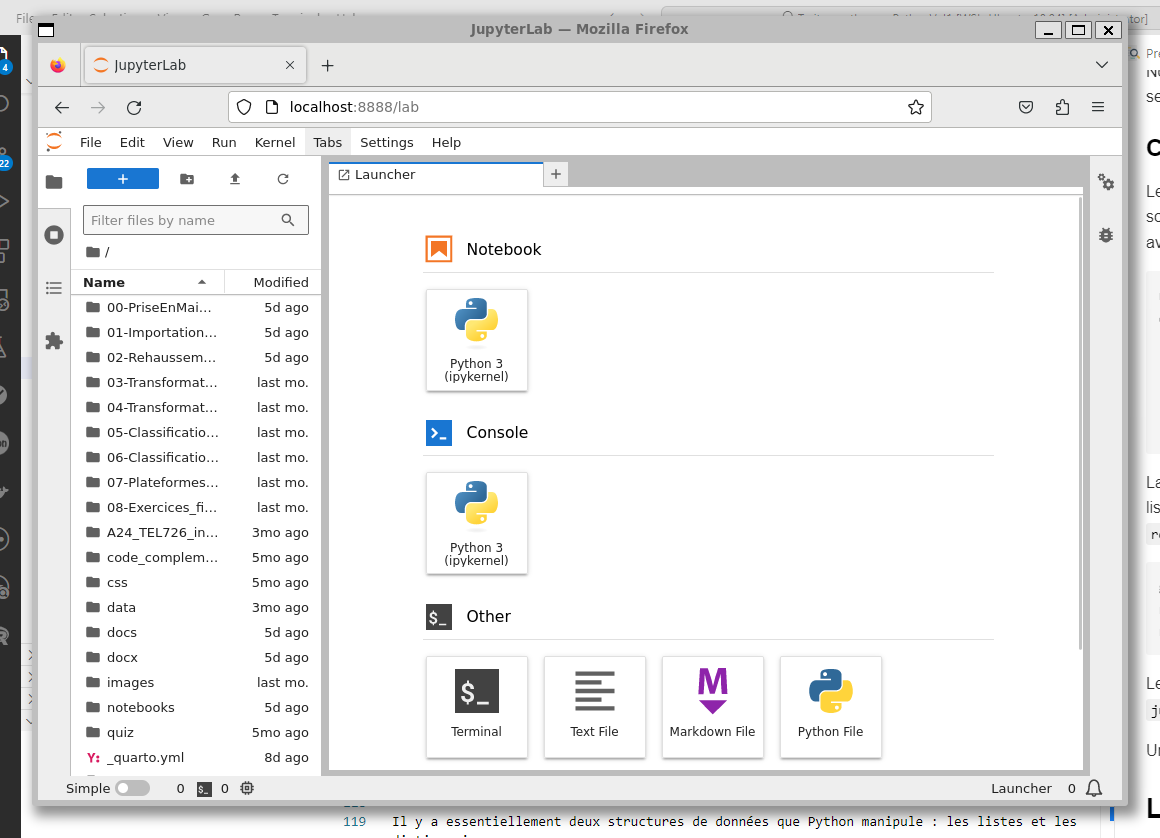
\includegraphics[keepaspectratio]{https://raw.githubusercontent.com/sfoucher/TraitementImagesPythonVol1/refs/heads/main/images/jupyter-accueil.png}}
\caption{Figure~1.1: La librairie NumPy est le fondement de nombreuses
librairies scientifiques (d'après
{(\href{references.html\#ref-NumpyNature}{Harris 2020})}).}
\end{figure}

\subsection{\texorpdfstring{{1.4} Les structures de base en
Python}{1.4 Les structures de base en Python}}\label{les-structures-de-base-en-python}

Il y a essentiellement deux structures de données que Python manipule :
les listes et les dictionnaires.

\subsubsection{\texorpdfstring{{1.4.1} Les
listes}{1.4.1 Les listes}}\label{les-listes}

Les listes sont comme des boites extensibles où vous pouvez ranger
différents types d'objets :

\begin{itemize}
\item
  Représentées par des crochets : \texttt{{[}1,\ 2,\ 3,\ "python"{]}}.
\item
  Ordonnées et modifiables (mutables), vous pouvez récupérer une valeur
  par sa position avec \texttt{{[}{]}}.
\item
  Permettent les doublons (deux fois la même valeur).
\item
  Idéales pour stocker des collections d'éléments que vous voulez
  modifier
\end{itemize}

\subsubsection{\texorpdfstring{{1.4.2} Les
tuples}{1.4.2 Les tuples}}\label{les-tuples}

Les tuples sont similaires aux listes, mais les boîtes sont scellées :

\begin{itemize}
\item
  Représentés par des parenthèses : \texttt{(1,\ 2,\ 3,\ "python")}.
\item
  Ordonnés mais non modifiables (immutables).
\item
  Permettent les doublons.
\item
  Souvent utilisé pour stocker des données qui ne doivent pas changer
  (comme des paramètres).
\end{itemize}

\subsubsection{\texorpdfstring{{1.4.3} Les ensembles
(Sets)}{1.4.3 Les ensembles (Sets)}}\label{les-ensembles-sets}

Les ensembles sont comme des boites magiques qui ne gardent qu'un
exemplaire de chaque objet :

\begin{itemize}
\item
  Représentés par des accolades : \texttt{\{1,\ 2,\ 3\}}.
\item
  Non ordonnés et modifiables.
\item
  N'autorisent pas les doublons.
\item
  Utiles pour éliminer les doublons et effectuer des opérations
  mathématiques sur des ensembles.
\end{itemize}

\subsection{\texorpdfstring{{1.5}
Dictionnaires}{1.5 Dictionnaires}}\label{dictionnaires}

Les dictionnaires sont comme des boites avec des étiquettes sur chcune
d'elle :

\begin{itemize}
\item
  Représentés par des accolades avec des paires clé-valeur :
  \texttt{\{"nom":\ "Python",\ "année":\ 1991\}}.
\item
  Non ordonnés et modifiables.
\item
  Les clés doivent être uniques, mais les valeurs peuvent être
  dupliquées
\item
  Utiles pour stocker des données associatives ou pour créer des tables
  de recherche rapide
\end{itemize}

\subsection{\texorpdfstring{{1.6} Programmation
objet}{1.6 Programmation objet}}\label{programmation-objet}

La programmation orientée objet (POO) en Python est comme construire
avec des blocs LEGO. Chaque objet est un bloc LEGO avec ses propres
caractéristiques (attributs) et capacités (méthodes). Les classes sont
les plans pour créer ces blocs. Par exemple, une classe ``Voiture''
pourrait avoir des attributs comme ``couleur'' et ``vitesse'', et des
méthodes comme ``démarrer'' et ``accélérer''.

Python rend la POO accessible avec des fonctionnalités conviviales :

\begin{enumerate}
\def\labelenumi{\arabic{enumi}.}
\item
  \textbf{Encapsulation} : Comme emballer un cadeau, elle cache les
  détails internes d'un objet.
\item
  \textbf{Héritage} : Permet de créer de nouvelles classes basées sur
  des classes existantes, comme un enfant héritant des traits de ses
  parents.
\item
  \textbf{Polymorphisme} : Permet à différents objets de répondre au
  même message de manière unique, comme si différents animaux
  répondaient différemment à ``fais du bruit''.
\end{enumerate}

Ces caractéristiques font de Python un excellent choix pour apprendre et
appliquer les concepts de la POO, rendant le code plus organisé et
réutilisable

\textbf{Liste des \emph{packages} utilisés dans ce chapitre}

\begin{itemize}
\tightlist
\item
  Pour importer et manipuler des fichiers géographiques~:

  \begin{itemize}
  \tightlist
  \item
    \texttt{numpy} pour manipuler des données matricielles.
  \item
    \texttt{rasterio} pour importer et manipuler des données
    matricielles.
  \end{itemize}
\item
  Pour construire des cartes et des graphiques~:

  \begin{itemize}
  \tightlist
  \item
    \texttt{tmap} est certainement le meilleur \emph{package} pour la
    cartographie.
  \item
    \texttt{ggplot2} pour construire des graphiques.
  \end{itemize}
\end{itemize}

\phantomsection\label{sec-016}
\subsection{\texorpdfstring{{1.7} Cahier de révision
(notebook)}{1.7 Cahier de révision (notebook)}}\label{cahier-de-ruxe9vision-notebook}

\phantomsection\label{refs}
\begin{CSLReferences}{1}{0}
\bibitem[\citeproctext]{ref-NumpyNature}
Harris, Millman, C. R. 2020. {«~Array programming with NumPy.~»}
\emph{{Nature}}: 357‑362.
\url{https://doi.org/10.1038/s41586-020-2649-2}.

\end{CSLReferences}

\end{document}
